\chapter{Algoritmer} \label{kap.algo}
Når man står med et problem inden for diskret matematik, er det første, man skal gøre at finde en model, der kan sætte problemet i matematisk kontekst. Denne model skal bestå af diskrete strukturer såsom funktioner, følger eller grafer, som vi omtalte i tidligere afsnit. Når man har opstillet en passende model til at løse problemet, skal man finde en metode, som kan løse det med denne model. Denne model skal helst tilpasses, så den kan løse det generelle problem. Det vil sige alle probemer af den type og form. Metoden skal bestå af en række trin, som slutteligt vil give resultatet. Disse trin kaldes en \emph{algoritme}. 
\begin{defn}
[Algoritmer] En algoritme er en begrænset mængde af præcist definerede instruktioner, der viser, hvordan et problem løses, eller hvordan en beregning udføres. 
\end{defn}

Der er dog nogle kendetegn, som man ønsker skal gøre sig gældende for den algoritme, man anvender til at løse sit problem. Herunder, at der optræder et input og et tilhørende, korrekt output. Algoritmens trin skal være præcist defineret, så der ikke er tvivl om, hvad der skal gøres i hvert trin. Det er derudover lettere at arbejde med algoritmer, som er \emph{begrænsede}, og dermed ikke har uendeligt mange trin. Algoritmen bør være effektiv, så man præcist og indenfor et begrænset tidsrum kan løse de forskellige trin. Slutteligt bør algoritmen være generel, så den er anvendelig på alle problemer af denne type og form.

I følgende afsnit vil vi skrive alle algoritmer i pseudokode, som er en forsimplet form for programmeringssprog. Pseudokode kan ikke direkte implementeres i nogen programmer, da det ikke har en bestemt syntaks. Grunden til at vi skriver algoritmerne i pseudokode, er, at det er nemt at omskrive til forskellige andre programmeringssprog.


\section{Algoritmetyper}
Der findes mange typer algoritmer, som løser mange forskellige problemer. Vi vil i det følgende se på forskellige typer af algoritmer.
\subsection{Søgealgoritmer}
\emph{Søgealgoritmer} bruges til at løse problemer, hvor man vil finde et element, $x$, i en liste $(a_{1}, a_{2}, \dotsc, a_{n})$, eller konkludere, at $x$ ikke er i listen. Her vil løsningen være $i$, hvis $x=a_{i}$. Det er altså indekset, der er løsningen. Der findes forskellige søgealgoritmer bl.a. \emph{den lineære søgning} og \emph{den binære søgning}. Ved den lineære søgning starter man med $a_1$ og ser, om $x=a_{1}$. Hvis dette er tilfældet, er $a_{1}$'s indeks svaret, men hvis $x \neq a_{1}$, fortsætter man til $a_{2}$ og så $a_{3}$. Sådan fortsætter man, indtil man finder et element i listen, der er lig $x$, hvis et sådant element eksisterer. Hvis dette er tilfældet, returnerer algoritmen elementets indeks og ellers returnerer den 0. \autoref{alg:lineaer} illustrerer et eksempel på en lineær søgealgoritme:

\begin{algorithm}[H] 
\caption{Den lineære søgealgoritme}
\begin{algorithmic}[1]

\Procedure{lineær søgning($x$: heltal, $a_{1},a_{2},\dotsc,a_{n}$: Heltal i listen)}{}
    \State $i:=1$
    \While{$i \leq n$ \textbf{and} $x \neq a_{i}$}
        \State $i:=i+1$
    \EndWhile
    \If{$i \leq n$} 
    \State \textbf{return} $lokation:=i$
    \Else
    \State \textbf{return} $lokation:=0$
    \EndIf
  \label{roy's loop}
\EndProcedure

\end{algorithmic}
\label{alg:lineaer}
\end{algorithm}


Modsat den lineære søgning kan den binære søgning kun bruges, når en liste er \emph{ordnet}. Det vil sige, hvis listen fx er voksende, aftagende eller alfabetisk, altså $(a_{1}<a_{2}<\dotsb<a_{n})$. Den binære søgealgoritme finder nu midten af listen, $a_{m}$, hvor $m=\left \lfloor \frac{n+1}{2} \right \rfloor$. $\lfloor \ \rfloor$ er flooroperatoren, der runder ned til første heltal. Vi ser nu, hvilken side det, vi søger, er på. Hvis $a_{m}<x$, tager vi halvdelen af listen, der er større end $a_{m}$ dvs: $(a_{m+1}, a_{m+2},\dotsc,a_{n})$. Ellers tager vi halvdelen mindre end og lig $a_{m}$: $(a_{1}, a_{2},\dotsc,a_{m})$. Når vi har vurderet hvilken side af midten, den værdi, vi søger, er på, deles denne halvdel på midten, hvorefter man igen skal vurdere, hvilken side man skal arbejde videre med. Dette fortsættes, indtil tallet er fundet. Den binære søgealgoritme er illustreret i \autoref{alg:binaer}.

\begin{algorithm}[H]
\caption{Den binære søgealgoritme}
\begin{algorithmic}[1]

\Procedure{binær søgning($x$: heltal, $a_{1},a_{2},\dotsc,a_{n}$: Voksende heltal i listen)}{}
    \State $i:=1$, \{$i$ er venstre endepunkt i søgeintervallet\}
    \State $j:=n$, \{$j$ er højre endepunkt i søgeintervallet\}
    \While{$i<j$}
        \State $m=\lfloor (i+j)/2 \rfloor$
    		\If{$x>a_{m}$}
    		\State $i:=m+1$
    		\Else
    		\State $j:=m$
    		\EndIf    
    \EndWhile
    \If {$x=a_{i}$}
    	\State \textbf{return} $lokation:=i$
    \Else
    	\State \textbf{return} $lokation:=0$
    \EndIf
  \label{roy's loop}
\EndProcedure

\end{algorithmic}
\label{alg:binaer}
\end{algorithm}

\subsection{Sorteringsalgoritmer} \label{kap:sortering}
Når vi arbejder med \emph{sorteringsalgoritmer}, er det, fordi vi ønsker at sortere en liste, således at den inddeles i fx voksende rækkefølge eller alfabetisk orden. Ligesom ved søgealgoritmerne er der flere forskellige sorteringsalgoritmer. Eksempler på disse er \emph{bubblesortering} og \emph{indskudssortering}. Bubblesortering er en af de simpleste sorteringsalgoritmer, men den er ikke så effektiv. Den sammenligner tilstødende værdier i en liste og bytter om på dem, hvis rækkefølgen ikke er korrekt. Vi vil komme ind på algoritmers effektivitet i \autoref{kap:kompleksitet}.

\begin{algorithm}[H]
\caption{Bubblesorteringsalgoritmen}
\begin{algorithmic}[1]

\Procedure{bubblesortering($a_{1},a_{2},\dotsc,a_{n}$: Reelle tal hvor $n \geq 2$)}{}
\EndProcedure
\For {$i:=1$ \textbf{to} $n-1$}
    	\For {$j:=1$ \textbf{to} $n-i$}
    		\If {$a_{j}>a_{j+1}$}
    			\State Ombyt $a_{j}$ og $a_{j+1}$ 	
\EndIf
\EndFor
\EndFor
\State $a_{1},a_{2},\dotsc,a_{n}$ er i voksende rækkefølge. 

\end{algorithmic}
\end{algorithm}

\begin{exmp}
Vi ser på en liste, $(3,4,2,5,1)$, som vi vil arrangere således, at den er i rækkefølge med stigende værdi. Algoritmen gentages fire gange, da listen har længden $n=5$, og algoritmen skal køre $n-1$ gange. 
\begin{align*}
	\text{Første gentagelse:} \qquad \qquad \qquad \quad \text{Anden 			gentagelse:} \qquad \qquad \qquad \quad \text{Tredje gentagelse:} 			\qquad \qquad \qquad \quad \\
	(\textbf{3,4},2,5,1) \rightarrow (\textbf{3,4},2,5,1) \qquad \qquad 		(\textbf{3,2},4,1,5) \rightarrow (\textbf{2,3},4,1,5) \qquad \qquad 		(\textbf{2,3},1,4,5) \rightarrow (\textbf{2,3},1,4,5) \qquad \qquad 		\\
	(3,\textbf{4,2},5,1) \rightarrow (3,\textbf{2,4},5,1) \qquad \qquad     	(2,\textbf{3,1},4,5) \rightarrow (2,\textbf{1,3},4,5) \qquad \qquad   	(2,\textbf{3,1},4,5) \rightarrow (2,\textbf{1,3},4,5) \qquad \qquad 		\\
	(3,2,\textbf{4,5},1) \rightarrow (3,2,\textbf{4,5},1) \qquad \qquad 		(2,1,\textbf{3,4},5) \rightarrow (2,1,\textbf{3,4},5) \qquad \qquad  	\qquad \qquad \qquad \qquad \qquad \qquad \qquad \quad \ \ \\
	(3,2,4,\textbf{5,1}) \rightarrow (3,2,4,\textbf{1,5}) \qquad \qquad 		\qquad \qquad \qquad \qquad \qquad \qquad \qquad \quad \ \  \qquad 			\qquad \qquad \qquad \qquad \qquad \qquad \quad \ \
\end{align*}

\begin{flushleft}
Fjerde gentagelse:
\\
$(\textbf{2,1},3,4,5) \rightarrow (\textbf{1,2},3,4,5)$
\end{flushleft}

Efter første gentagelse har algoitmen placeres det største tal bagerst i listen, efter anden gentagelse har algoritmen placeret det næst største tal på næst sidste plads i listen. Således fortsætter algoritmen indtil listen er i korrekt rækkefølge.

\end{exmp}

Indskudssortering er på samme måde som bubblesortering simpel og til tider ineffektiv. For denne algoritme gælder det, at man starter med den anden værdi i listen, som sammenlignes med den første værdi. Disse to sorteres nu efter størrelse. Den tredje værdi i listen sammenlignes derefter med den første. Hvis den er større, sammenlignes den med den anden værdi i listen, og på den måde sorteres hele rækken, så de til sidst står i rækkefølge.

\begin{algorithm}[H]
\caption{Indskudssorteringsalgoritmen}
\begin{algorithmic}[1]

\Procedure{indskudssortering($a_{1},a_{2},\dotsc,a_{n}$: Reelle tal hvor $n \geq 2$)}{}
\EndProcedure
\For {$j:=2$ \textbf{to} $n$}
	\State $i:=1$
    	\While {$a_{j}>a_{i}$}
    		\State $i:=i+1$
    	\EndWhile
    	\State $m:=a_{j}$
    	\For {$k:=0$ \textbf{to} $j-i-1$}
    		\State $a_{j-k}:=a_{j-k-1}$
    	\EndFor
    	\State $a_{i}:=m$
\EndFor
\State $a_{1},a_{2},\dotsc,a_{n}$ er i voksende rækkefølge. 

\end{algorithmic}
\end{algorithm}

\begin{exmp}
Vi ser igen på en liste, $(3,4,2,5,1)$, som vi gerne vil sortere i rækkefølge, således at de står med stigende værdi. Til at gøre dette, vil vi bruge indskudssorteringsalgoritmen. Illustrationen, som ses nedenfor, viser, at alle understregede tal står i korrekt rækkefølge. Tallet markeret med fed er det næste tal, som algoritmen skal placere i den korrekte liste.

\begin{figure}[H]
\label{fig:indskud}
	\begin{flushleft}
	$i=1: \ (\underline{3},\textbf{4},2,5,1) \rightarrow (\textbf{4}, \underline{3},2,5,1)\rightarrow (\underline{3,\textbf{4}},2,5,1)$ \\
	$i=2: \ (\underline{3,4},\textbf{2},5,1) \rightarrow (\underline{\textbf{2},3,4},5,1) $\\
	$i=3: \ (\underline{2,3,4},\textbf{5},1) \rightarrow (\textbf{5},\underline{2,3,4},1) \rightarrow (\underline{2}, \textbf{5},\underline{3,4},1) \rightarrow (\underline{2,3}, \textbf{5}, \underline{4},1) \rightarrow (\underline{2,3,4,\textbf{5}},1) $ \\
	$i=4: \ (\underline{2,3,4,5},\textbf{1}) \rightarrow (\underline{\textbf{1},2,3,4,5}) $\\
 	\end{flushleft}
\end{figure}

Vi kan se, at algoritmen starter med at sammenligne fire med tre. Den tjekker først om fire er mindre end tre. Da det er større og der ikke er flere tal i listen, placeres fire i slutningen af den korrekte liste. Den tjekker nu det tredje tal i listen og ser med det samme, at det er mindre end det første tal i den korrekte liste. Derfor placeres to på den første plads i den korrekte liste. Den sammenligner nu fem med alle tal i den korrekte liste, og placerer fem efter det største tal den er større end. Dette gør den med alle tallene i listen, og den har til sidst placeret alle tallene i listen i korrekt rækkefølge.


\end{exmp}
\subsection{Grådige algoritmer}
Når man arbejder med optimeringsproblemer, som omhandler minimering eller maksimering, som fx kunne være at finde den længste eller korteste vej i en graf, kan man ofte bruge \emph{grådige algoritmer}.
En grådig algoritme vælger altid det \emph{lokalt optimale} valg og antager, at dette medfører en \emph{global optimal} løsning, altså den bedst mulige løsning. Det lokalt optimale valg findes ved at vælge den umiddelbart bedste løsning for hvert muligt trin.
I mange tilfælde vil dette lede til global optimering, men der kan også forekomme situationer, hvor algoritmen vil finde en suboptimal løsning. Ligegyldigt om algoritmen finder en optimal eller suboptimal løsning, kalder vi den en grådig algoritme. 
   
\autoref{fig:greedy.eks} er et eksempel på en grådig algoritme, som har forsøgt at finde den længst mulige simple vej i en graf.

\begin{figure}[H]
\centering
	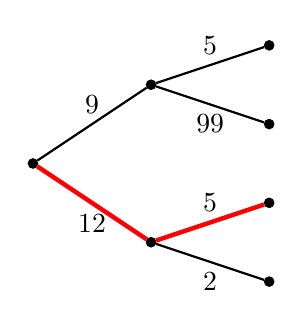
\begin{tikzpicture}

      \tikzset{enclosed/.style={draw, circle, inner sep=0pt, minimum size=.12cm, fill=black}}
% Vertices
      	\node[enclosed] (v1) at (0,2) {};
      	\node[enclosed] (v2) at (1.5,1) {};
    	\node[enclosed] (v3) at (1.5,3) {};
  	    \node[enclosed] (v4) at (3,0.5) {};
  	    \node[enclosed] (v5) at (3,1.5) {};
  	    \node[enclosed] (v6) at (3,3.5) {};
  	    \node[enclosed] (v7) at (3,2.5) {};    
%Edges
		\path[ultra thick] (v1) edge[red] node[midway, below, black] {$12$} (v2);
		\path[thick] (v1) edge node[midway, above] {$9$} (v3);
		\path[thick] (v2) edge[red, ultra thick] node[midway, above, black] {$5$} (v5);
		\path[thick] (v2) edge node[midway, below] {$2$} (v4);
		\path[thick] (v3) edge node[midway, above] {$5$} (v6);
		\path (v3) edge[thick] node[midway, below] {$99$} (v7);


	\end{tikzpicture}
	\caption{Længste vej, i simpel graf, ifølge grådig algoritme.}
	\label{fig:greedy.eks}
\end{figure}

Vi kan se, at algoritmen har valgt de lokalt optimale valg, men den har ikke fundet den globalt optimale løsning. Det er tydeligt at se, at denne algoritme ikke er pålidelig nok til at løse sådanne problemer, da den ikke konsekvent finder den globalt optimale løsning. Der findes dog nogle grådige algoritmer, som er optimeret, så de altid finder den globalt optimale løsning, så længe grafen overholder specifikke krav. Dette ser vi i \autoref{kap:dijkstras}.

    

\begin{exmp}
Det danske møntsystem har seks forskellige mønter med værdier på $0.5,\ 1,\ 2,\ 5,\ 10$ og $20$ kroner. Systemet er optimeret således, at man kan lave byttepenge vha. en grådig algoritme. Man kan altid finde den optimale løsning ved først at tage så mange som muligt af de mest værdifulde mønter, og derefter tager man så mange som muligt af de næstmest værdifulde mønter. Man fortsætter denne proces, indtil man har den ønskede mængde byttepenge.
\begin{algorithm} [H] 
\caption{Grådig algoritme til byttepenge}
\label{alg:byt}
\begin{algorithmic}[1]

\Procedure{Byttepenge($c_1,c_2,\dotsc,c_r$: værdien af mønter, hvor $c_1>c_2>\dotsb >c_r;n:$ et positivt heltal)}{}
\EndProcedure
\For{$i:=1$ \textbf{to} $r$}
    \State $d_i:=0$ ($d_i$ tæller mængden af mønter med værdi $c_i$)
    \While{$n \geq c_i$}
    	\State $d_i := d_i+1$ (Mængden af mønter med værdi $c_i$ øges med en.)
    	\State $n := n-c_i$
\EndWhile
\EndFor
\State ($d_i$ er mængden af mønter med værdi $c_i$ for $i=1,2,\dotsc,r$)
\end{algorithmic}
\end{algorithm}
Denne algoritme vil altid vælge den globalt optimale løsning i dette specifikke problem. Der kan dog være problemer, hvis mønternes værdi ændrer sig. 
Vi forestiller os nu, at vi har et møntsystem udelukkende med tre mønter af værdi $25$, $10$ og $1$. Der opstilles her et problem, hvor vi vil have $30$ kroner i byttepenge. \autoref{alg:byt} vil nu få en løsning, som bruger én mønt af værdi $25$ og fem mønter af værdi $1$. Dette er en suboptimal løsning, da man kunne have brugt tre mønter af værdi $10$.
Dette viser, at grådige algoritmer ikke altid finder den optimale løsning.
\end{exmp}


\section{Dijkstras algoritme}
I \ref{defn:min.vej} definerede vi distancen af den korteste vej i en vægtet graf. For at finde den korteste vej vil vi anvende \emph{Dijkstras algoritme}. Dijkstras algoritme kan bruges til at finde den korteste vej i en simpel, vægtet graf, hvori vægtene for alle kanter i grafen skal være ikke-negative. Algoritmen fungerer således, at den finder den korteste vej fra en startknude, $v_{1}$, til en endeknude, $v_{m}$, ved først at finde naboknuderne til $v_{1}$ og undersøge hvilken af disse, der har den mindste distanceværdi og altså er tættest på startknuden. Derefter tager den udgangspunkt i den naboknude, hvortil distanceværdien er mindst og fortsætter ad dennes vej, så længe denne vej har en mindre distanceværdi end en alternativ vej. Fremgangsmåden vil her illustreres ved hjælp af et eksempel, som tager udgangspunkt i \ref{kap:grafteori}.

\begin{exmp} \label{exmp.dijkstae}
Betragt figur \ref{fig.dijkstraexmp}
\begin{figure}[H]
\centering
	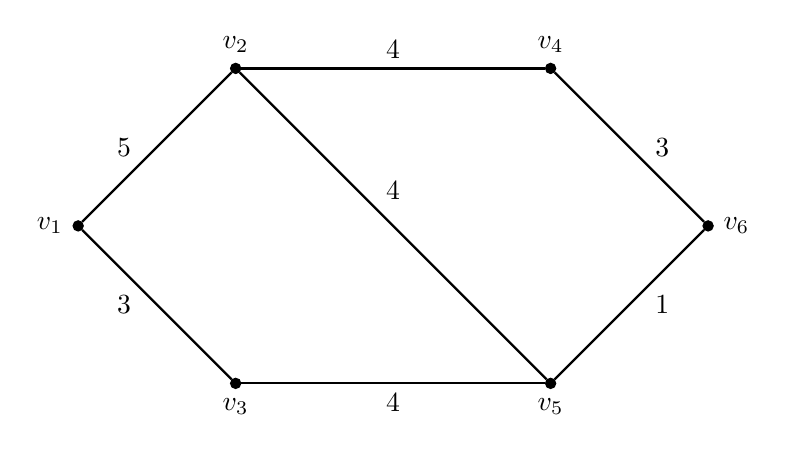
\begin{tikzpicture}

      \tikzset{enclosed/.style={draw, circle, inner sep=0pt, minimum size=.13cm, fill=black}}
%% Vertices
      	\node[enclosed, label={left: $v_1$}] (v1) at (0,2) {};
      	\node[enclosed, label={above: $v_2$}] (v2) at (2,4) {};
    	\node[enclosed, label={below: $v_3$}] (v3) at (2,0) {};
  	    \node[enclosed, label={above: $v_4$}] (v4) at (6,4) {};
     	\node[enclosed, label={below: $v_5$}] (v5) at (6,0) {};
     	\node[enclosed, label={right: $v_6$}] (v6) at (8,2) {};
%Edges
		\path [-, > = latex, thick] (v1) edge node[midway, left=2mm] {$ 5 $} (v2);
		\path [-, > = latex, thick] (v1) edge node[midway, left=2mm] {$ 3 $} (v3);
		\path [-, > = latex, thick] (v2) edge node[midway, above] {$ 4 $} (v4);
		\path [-, > = latex, thick] (v2) edge node[midway, above=2mm] {$ 4 $} (v5);
		\path [-, > = latex, thick] (v3) edge node[midway, below] {$ 4 $} (v5);
		\path [-, > = latex, thick] (v4) edge node[midway, right=2mm] {$ 3 $} (v6);
		\path [-, > = latex, thick] (v5) edge node[midway, right=2mm] {$ 1 $} (v6);

	\end{tikzpicture}
	\caption{Simpel, vægtet graf.}
	\label{fig.dijkstraexmp}
\end{figure}
I figur \ref{fig.dijkstraexmp} vil vi finde den korteste vej fra $v_{1}$ til $v_{6}$. Dijkstras algoritme vil gøre dette ved at finde den korteste vej fra startknuden, $v_{1}$, til hver knude, indtil den når endeknuden, $v_{6}$. Først vil den se, at startknuden har naboknuderne $v_{2}$ og $v_{3}$. Der er altså to veje fra startknuden, $P=(v_{1},v_{2})$ med distancen 5 og $P=(v_{1},v_{3})$ med distancen 3. Dermed er $v_{3}$ den knude, der er tættest på startknuden. Herefter er der igen to veje, $P=(v_{1},v_{2})$ med distancen 5 og $P=(v_{1},v_{3},v_{5})$ med distancen 7. Den første af disse vælges, da denne har den mindste distance, og $v_{2}$ er dermed knuden, som er næsttættest på startknuden. Nu er der tre forskellige veje, $P=(v_{1},v_{2}, v_{4})$ med distancen 9, $P=(v_{1},v_{2}, v_{5})$ med distancen 9 og $P=(v_{1},v_{3}, v_{5})$ med distancen 7. Den tredje vælges, og det er nu noteret, at den korteste vej fra $v_{1}$ til $v_{5}$ har distancen 7. Der er nu igen kun to mulige veje at vælge imellem, $P=(v_{1},v_{2}, v_{4})$ med distancen 9 og $P=(v_{1},v_{3}, v_{5}, v_{6})$ med distancen 8. $P=(v_{1},v_{2}, v_{5})$ er ikke længere en mulig vej, da vi allerede har fundet den korteste vej fra $v_{1}$ til $v_{5}$. Den anden vej har den mindste distance, og derfor vælger vi denne, og vi ved nu, at den korteste vej fra $v_{1}$ til $v_{6}$ er $P=(v_{1},v_{3}, v_{5}, v_{6})$ og har distancen 8.
\end{exmp}
Ovenstående eksempel er simpelt og kan hurtigt løses ved fx brute force metoden, men i større og mere komplicerede grafer er Dijkstras algoritme meget mere effektiv. For at skabe yderligere overblik over hvordan Dijkstras algoritme fungerer, vil vi her gå i dybden med dennes mere teoretiske del.
\begin{algorithm}[H]
\caption{Dijkstras algoritme}
\begin{algorithmic}[1]

\Procedure{dijkstra($G$: vægtet, forbundet, simpel graf med kun ikke-negative vægte)}{}
    \State \{$G$ {har knuderne $a = v_{1}, v_{2}, \dotsc, v_{m} = z$ og vægtene til kanterne $w(v_{i}, v_{j})$, hvor $w(v_{i}, v_{j}) = \infty$ hvis {$(v_{i}, v_{j})$} ikke er en kant i G\}}
	\For {$i := 2$ \textbf{to} $n$}
		\State $L(v_{i}) := \infty$
	\EndFor
	\State $L(a) := 0$	
	\State $S := \emptyset$
	\State {\{distancen til hver knude initialiseres, så $a = 0$, og distancen til alle andre knuder er $\infty$, derudover er $S$ defineret som en tom mængde\}}
    \While{$z \notin S$}
        \State {$u :=$ en knude som ikke er i $S$ med $L(u)$ som minimum}
        \State $S := S \cup \{u\}$
        \For {alle $v \notin S$}
        	\If {$L(u) + w(u,v) < L(v)$} {$L(v) := L(u) + w(u,v)$}
        	\State \{dette tilføjer knuder til $S$ med minimal 			distance og opdaterer distancerne til
        	\State knuderne, som ikke er i $S$\}
        	\EndIf
    	\EndFor
    \EndWhile
    \State {\textbf{return} $L(z)$ \{$L(z)$ er distancen af den korteste vej fra $a$ til $z$\}} 
\EndProcedure

\end{algorithmic}
\label{alg:dijkstra}
\end{algorithm}
Det første, der sker, er, at startknuden noteres som $0$, altså $v_{1} = 0$, og resten af knuderne noteres som $\infty$. Her betegnes den korteste vej som $\alpha_{k}(v_1,v_m)$, fra definition \ref{defn:min.vej}, hvor $k$ er antallet af \emph{iterationer} gennemført i algoritmen. Antallet af iterationer er det antal gange en løkke gennemkøres, altså hver gang vejen opdateres.  $\alpha_{0}(v_1,v_1)$ betyder altså, at vi har nul iterationer og dermed kun kender startknuden med distancen 0. Derudover oprettes en mængde $S$, for hvilken det gælder, at $S = \emptyset$ når $k = 0$. Ved første iteration undersøges startknudens naboknuder, og man bestemmer, som i eksemplet ovenfor, hvilken distance er mindst. Dermed er startknudens nærmeste knude fundet, og denne tilføjes nu til mængden $S$. For hver iteration tilføjes et nyt element til mængden, og denne proces fortsætter, til algoritmen har fundet den korteste vej fra startknuden til endeknuden. Mængden, $S$, indeholder til sidst distancerne for den korteste vej fra startknuden til alle knuder i grafen. 



\section{Kompleksitet}
%side 250 ish
%table 1 side 247 i pdf.

Der findes to former for kompleksitet, men vi vælger at fokusere på tidskompleksitet. Den anden form for kompleksitet er pladskompleksitet. 
Der er tre former for tilfælde: bedste, værste og gennemsnitlige. 
I bedste tilfælde ser man på det laveste antal trin for en inputstørrelse, $n$. I værste ser man på det højeste og i gennemsnittet, det gennemsnitlige. 
\emph{Bedste tilfælde} beskriver algoritmen under optimale forhold, i en lineær søgealgoritme vil dette altså være, at elementet der søges efter, er det første element i listen. 
Oftere ser man på enten \emph{værste tilfælde} eller \emph{gennemsnitlige tilfælde}. 
Det gennemsnitlige tilfælde vil give et rigtigt godt overblik over hvor god algoritmen er, dog er det meget svært at bestemme hvad et gennemsnitligt input er, da det er svært at bestemme nogle parametre at vælge ud fra. 
Det værste tilfælde giver et godt overblik over hvor lang tid det kan tage. Ved man at algoritmen er lineær i værste tilfælde, vil man kunne løse den i rimelig tid for alle størrelser $n$.
De forskellige resultater i vores analyse af algoritmerne, kan deles op i kategorier, de mest gængse er: $\log n$, $\sqrt{n}$, $n$, $n^x$, $x^n$ og $n!$, men det kan også være en kombination af disse, som $n!n$, $n\log n$ eller lignende.
For at beskrive disse algoritmer i fx værste tilfælde, vil man bruge operatorerne \emph{store-O}, \emph{store-Omega} og \emph{Theta}. Man vil her fokusere på \emph{asymptotiske $n$-værdier}, altså ved rigtigt store værdier for $n$, da man i nogle tilfælde vil have en algoritme der er langsommere end den øvre bindende funktion ved små $n$, men ved større, som fx over 10.000, er hurtigere.

\subsection{store-$O$}
\begin{defn}
$f(n) = O(g(x))$ hvis og kun hvis $\exists$ positive konstanter $C$ og $n_o$ så at $f(n) \leq C g(n) \forall n \geq n_o$
\end{defn}

Store-$O$ bliver brugt til at binde funktionen opadtil, begrænse den oppe fra. Man kan med garanti sige, at algoritmen tager store-$O$ tid eller mindre. 
\begin{exmp}
\begin{align*}
f(n)=& 13n+3 \\
13n+3 \leq& 20n \forall \ n \geq 1 \\
f(n) =& O(n)
\end{align*}
\end{exmp}
Man vil også kunne sige, at $f(n)$ er mindre end $n!$ eller en anden vilkårlig højere funktion $g(n)$, men da man altid vil vælge den mest begrænsende funktion, vil $n$ være det mest præcise. 

\subsection{Store-$\Omega$}
\begin{defn}
$f(n) = \Omega(g(n))$ hvis og kun hvis $\exists$ positive konstanter $C$ og $n_o$ så at $f(n) \geq C g(n) \forall n \geq n_o$
\end{defn}
Store-Omega bruges, omvendt store-$O$, til at binde funktionen nedadtil, altså finde den nedre grænse for algoritmen, den vil mindst tage store-Omega tid i det givne tilfælde.
\begin{exmp}
\begin{align*}
f(n)=& 13n+3 \\
13n+3 \geq& n \forall \ n \geq 1 \\
f(n) =& \Omega(n)
\end{align*}
\end{exmp}

På samme måde som ved store-$O$-notationen, vil man her kunne vælge en vilkårlig mindre funktion, $logn$, $1$ med flere, men da man vil begrænse den så meget som muligt, vælger man den største funktion $g(n)$ hvor uligheden stadig er sand.
\subsection{Theta}
\begin{defn}
$f(n) = \Theta(g(x))$ hvis og kun hvis $\exists$ positive konstanter $C_1, C_2$ og $n_o$ så at $C_1g(n) \leq f(n) \leq C_2g(n) \forall n \geq n_o$
\end{defn}
Når man har fundet den øvre og den nedre grænse, store-O og store-Omega, kan man finde Theta, den tætte bundne funktion,
\begin{exmp}
\begin{align*}
f(n)=& 13n+3 \\
n \leq 13n+3 \leq& 10n \forall \ n \geq 1 \\
f(n) =& \Theta(n)
\end{align*}
\end{exmp}
P \\
NP \\
NP-Complete \\
NP-Hard. 

Store-O
O
Store-Omega

Theta
store-Theta

\pgfplotsset{compat=1.10}
\usepgfplotslibrary{fillbetween}

\begin{figure}[H]
\centering
	\begin{tikzpicture}
\begin{axis}[
    xmin=0, xmax=10,
    ymin=0, ymax=10
    ]

    \addplot [name path=plot1, ultra thin, domain=-10:10, samples=150]{x^2};
    \addplot [name path=plot2, ultra thin, domain=-10:10, samples=150]{2*x+4};


\end{axis}
	\end{tikzpicture}
	\caption{Kompleksitet}
	\label{fig.kompleksitet}
\end{figure}